\documentclass[11pt,letterpaper]{article}
\usepackage[utf8]{inputenc}
\usepackage{graphicx}
\usepackage{amsmath}
\usepackage{amsfonts}
\usepackage{amssymb}
\usepackage{float} %necessary to make [H] work for figures (place in text)
\usepackage{subfig}
\title{(yeaheyah)}
\author{Pawe\l{} Janowski}
\setlength{\topmargin}{0in}
\setlength{\headheight}{0in}
\setlength{\headsep}{0in}
\setlength{\textheight}{9in}
\setlength{\oddsidemargin}{0in}
\setlength{\textwidth}{6.5in}
%\usepackage{fullpage}
\parskip 8pt
\usepackage{Sweave}
\begin{document}
\setkeys{Gin}{width=0.5\textwidth}
\begin{flushright}
\parskip 0pt
Pawe\l{} Janowski
 
\today
\vspace{10 mm}
\end{flushright}
\begin{center}
\begin{Large}
\textbf{Basic Applied Statistics
Midterm \#2}
\vspace{10 mm}
\end{Large}
\end{center}


\begin{enumerate}
\item Problem 1 \\
a.\\
\begin{Schunk}
\begin{Sinput}
> boxplot(intake, horizontal = TRUE)
\end{Sinput}
\end{Schunk}
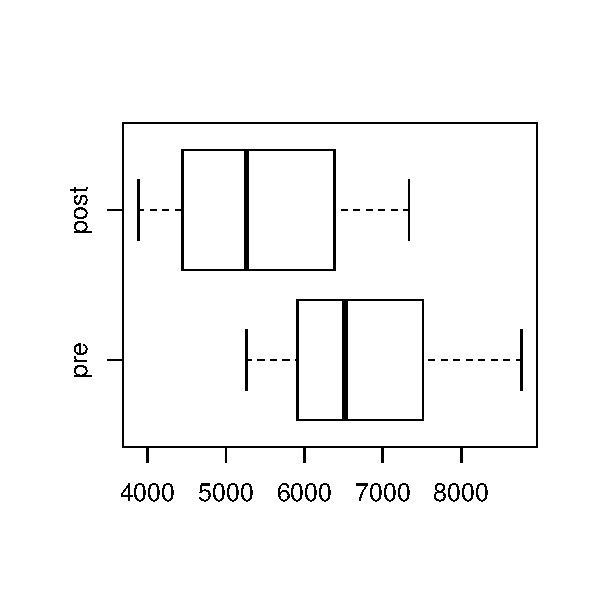
\includegraphics{midterm2-001}
\\

b.\\
\begin{Schunk}
\begin{Sinput}
> x = (intake$pre - intake$post)
> qqnorm(x)
> qqline(x)
\end{Sinput}
\end{Schunk}
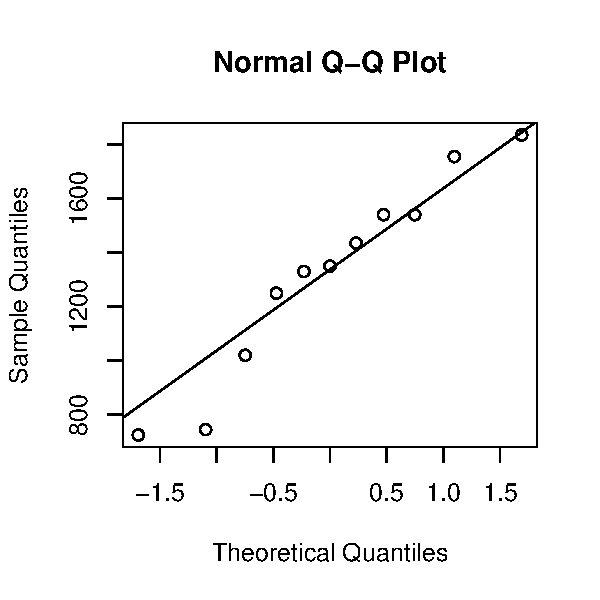
\includegraphics{midterm2-002}
\\
The qqplot is not perfect but it also isn't terrible so I would say yes, it is at least plausible that the distribution of the differences is normal.\\
\\

c.\\
$\mu_1=$premenstrual intake\\
$\mu_2=$postmenstrual intake\\
$H_0:\mu_2-\mu_1=0$
$H_a:\mu_2-\mu_1<0$
\begin{Schunk}
\begin{Sinput}
> t.test(intake$post, intake$pre, alt = "less")
\end{Sinput}
\begin{Soutput}
	Welch Two Sample t-test

data:  intake$post and intake$pre 
t = -2.6242, df = 19.92, p-value = 0.008143
alternative hypothesis: true difference in means is less than 0 
95 percent confidence interval:
      -Inf -452.4367 
sample estimates:
mean of x mean of y 
 5433.182  6753.636 
\end{Soutput}
\end{Schunk}
The p-value is .008 so even at a 99 \% significance level we can reject the hypothesis: there is sufficient evidence to believe that the postmenstrual intake is lower than premenstrual intake.\\

\item Problem 2
\begin{Schunk}
\begin{Sinput}
> mod2 = aov(time ~ poison + treat + poison * treat, data = rats)
> summary(mod2)
\end{Sinput}
\begin{Soutput}
             Df  Sum Sq Mean Sq F value    Pr(>F)    
poison        2 1.03301 0.51651 23.2217 3.331e-07 ***
treat         3 0.92121 0.30707 13.8056 3.777e-06 ***
poison:treat  6 0.25014 0.04169  1.8743    0.1123    
Residuals    36 0.80073 0.02224                      
---
Signif. codes:  0 ‘***’ 0.001 ‘**’ 0.01 ‘*’ 0.05 ‘.’ 0.1 ‘ ’ 1 
\end{Soutput}
\end{Schunk}
\begin{Schunk}
\begin{Sinput}
> plot(mod2, which = 2)
\end{Sinput}
\end{Schunk}
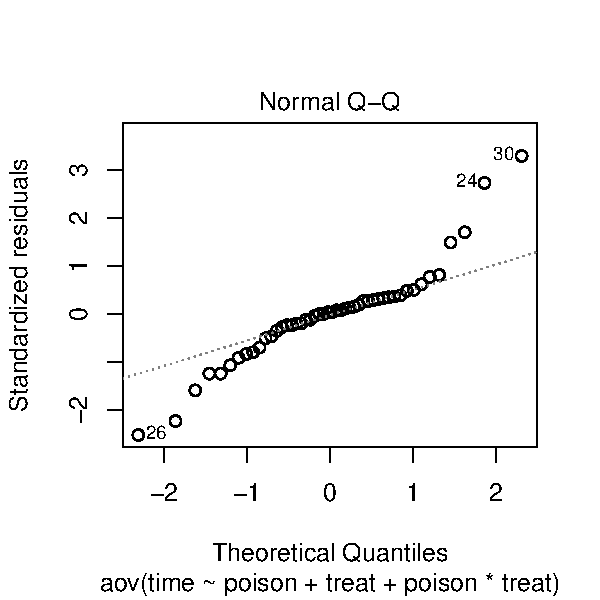
\includegraphics{midterm2-005}
\begin{Schunk}
\begin{Sinput}
> plot(mod2, which = 1)
\end{Sinput}
\end{Schunk}
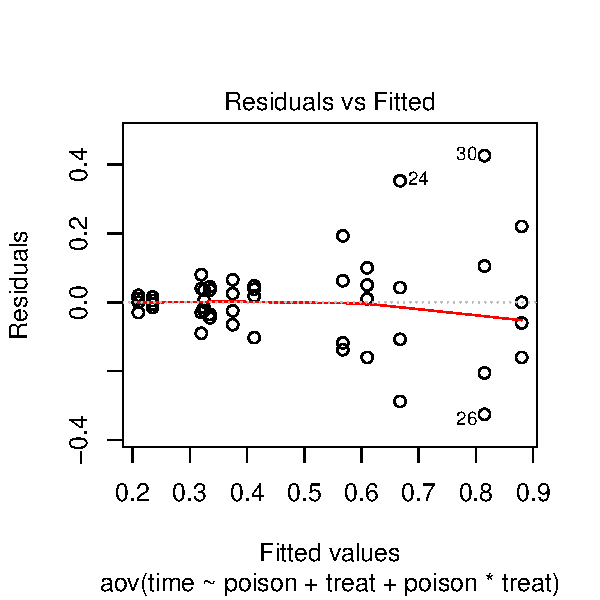
\includegraphics{midterm2-006}
The Two-Factor ANOVA test results in a high p-value for the interaction effects so we can accept that there is no interaction between the two factors. On the other hand the p-values for both poison and treatment are very low so at any reasonable significance level we can accept that time depends on both the poison and the treatment.

Nevertheless, plots of residuals are shed some doubt on the test and on the normality and constant variance assumptions. In this case I would maybe doubt the results of anova (thought the p-values are really low so probably the dependence conclusion is valid). However, I would seek some other method to make sure.

\begin{Schunk}
\begin{Sinput}
> TukeyHSD(mod2, which = "treat")
\end{Sinput}
\begin{Soutput}
  Tukey multiple comparisons of means
    95% family-wise confidence level

Fit: aov(formula = time ~ poison + treat + poison * treat, data = rats)

$treat
           diff         lwr         upr     p adj
B-A  0.36250000  0.19852116  0.52647884 0.0000047
C-A  0.07833333 -0.08564550  0.24231217 0.5772283
D-A  0.22000000  0.05602116  0.38397884 0.0048556
C-B -0.28416667 -0.44814550 -0.12018783 0.0002333
D-B -0.14250000 -0.30647884  0.02147884 0.1077087
D-C  0.14166667 -0.02231217  0.30564550 0.1107678
\end{Soutput}
\end{Schunk}
A \; C \; D \; B\\
|\_\_\_\_\\
| \; \ \ \ \_\_\_\_\\
| \quad      \_\_\_\_\\
\\
This should be staggered. I can't make these lines yet in latex.
\begin{Schunk}
\begin{Sinput}
> TukeyHSD(mod2, which = "poison")
\end{Sinput}
\begin{Soutput}
  Tukey multiple comparisons of means
    95% family-wise confidence level

Fit: aov(formula = time ~ poison + treat + poison * treat, data = rats)

$poison
            diff        lwr         upr     p adj
II-I   -0.073125 -0.2020091  0.05575913 0.3583151
III-I  -0.341250 -0.4701341 -0.21236587 0.0000005
III-II -0.268125 -0.3970091 -0.13924087 0.0000339
\end{Soutput}
\end{Schunk}
3 \; 2 \; 1\\
| \; \ \ \ \_\_\_\_\\
Poison 3 differs from 1 and 2 but 1 and 2 don't differ from each other.

\item Problem 3
\begin{Schunk}
\begin{Sinput}
> t.test(vital.capacity ~ group, data = vitcap, alt = "less")
\end{Sinput}
\begin{Soutput}
	Welch Two Sample t-test

data:  vital.capacity by group 
t = -2.9228, df = 19.019, p-value = 0.004362
alternative hypothesis: true difference in means is less than 0 
95 percent confidence interval:
       -Inf -0.4261231 
sample estimates:
mean in group 1 mean in group 3 
       3.949167        4.992500 
\end{Soutput}
\end{Schunk}
According to these results the null hypothesis can be rejected at any reasonable significance level: there is evidence to support the belief that vital capacity of group 1 (exposed>10 years) workers is less than the vital capacity of not exposed workers (group2). Howevever this data is misleading for two reasons: first the data provided is just a subset of a much larger data set, so it is selected we don't know by which criteria and does not provide all the data. Second, more importantly, there is a second factor which is age: all of the group 1 workers are much older than the group 3 workers, so that may play a role in influencing the vital capacity. A better test would be using group 3 workers who have a mean age equal to the group 1 workers.

\end{enumerate}
\end{document}
